\documentclass[conference]{IEEEtran}
\usepackage[ngerman]{babel}
\usepackage[utf8]{inputenc}
\usepackage[T1]{fontenc}
\usepackage{graphicx}
\usepackage{caption}
\usepackage{subcaption}

\begin{document}
\title{Netzwerk-Service-Assurance-Tests über verteilte Systeme auf dem
TU Clausthal Campus}
\author{\IEEEauthorblockN{Christian Rebischke}
\IEEEauthorblockA{Technische Universität Clausthal\\
Rechenzentrum\\
Email: Christian.Rebischke@tu-clausthal.de}}

\maketitle

\begin{abstract}
Um eine gleichbleibende Netzqualität innerhalb des Netzes der
TU Clausthal zu gewährleisten, werden Computersysteme auf dem
Campus verteilt, um Service-Assurance-Tests durchzuführen. Diese
Tests sollen eine gleichbleibende und stabile Verbindung garantieren
und beim Abweichen von Messergebnissen einen Netzwerkadministrator
alarmieren. Die Ergebnisse sollen in einer Datenbank gespeichert und
für die weitere Verwertung gefiltert und optimiert
werden. Dabei ist geplant, die Masse an Computersystemen mit
State-of-the-Art-Orchestration und Config-Management-Tools im
Schwarm zu administrieren.
\end{abstract}

\IEEEpeerreviewmaketitle

\section*{Problemstellung}
Das Netz der TU Clausthal erstreckt sich über mehrere Standorte.
Teilweise liegen diese Standorte nicht in Clausthal selbst, wie
beispielsweise das EFZN in Goslar. Dementsprechend schwierig gestaltet
sich die Wartung und der Betrieb des Netzes. So kann auf Netzeinbrüche
etwa nur reaktiv nach Meldung des Problems reagiert werden. Das
Aufspüren der Ursache ist ebenfalls nur manuell und mit viel Aufwand
möglich. Ein modernes Monitoring von zugesicherten Bandbreiten findet
demnach nicht statt. Es kann also zwar eine Anbindung, aber keine
stabile und gleichbleibende Bandbreite über einen längeren Zeitraum
garantiert werden, wie es in größeren Betrieben seit geraumer Zeit mit
Service-Level-Agreements der Fall ist.
\section*{Lösungsansatz}
Um erste Service-Level-Agreements zu etablieren gilt es die Grundlage
dafür zu schaffen: Service-Assurance-Tests. Die Service-Assurance-Tests
sollen ein Monitoring der Netzqualität ermöglichen und Probleme erkennen
bevor schwerwiegendere Ereignisse auftreten oder die Nutzer des
Netzwerks auf Qualitätseinbußen aufmerksam werden. Die Implementierung
der Tests erfolgt mit einer gängigen Programmiersprache und unter
Beachtung des RFC2544 (Request for Comments 2544) der IETF (Internet
Engineering Task Force) und den darauf aufbauenden Industriestandard
ITU-T Y.1564.  Zur besseren Skalierbarkeit werden diese
Service-Assurance-Tests auf Computersystemen platziert. Diese
Computersysteme können dann auf dem Campus verteilt werden und
sollen sich von einem Command-and-Control-Server im Schwarm
administrieren lassen. Dafür werden moderne Config-Management-Tools
eingesetzt werden. Die von den Computersystemen gewonnenen Daten
sollen in einer Datenbank abgespeichert und grafisch aufgewertet werden.
\begin{figure}[h]
    \centering
    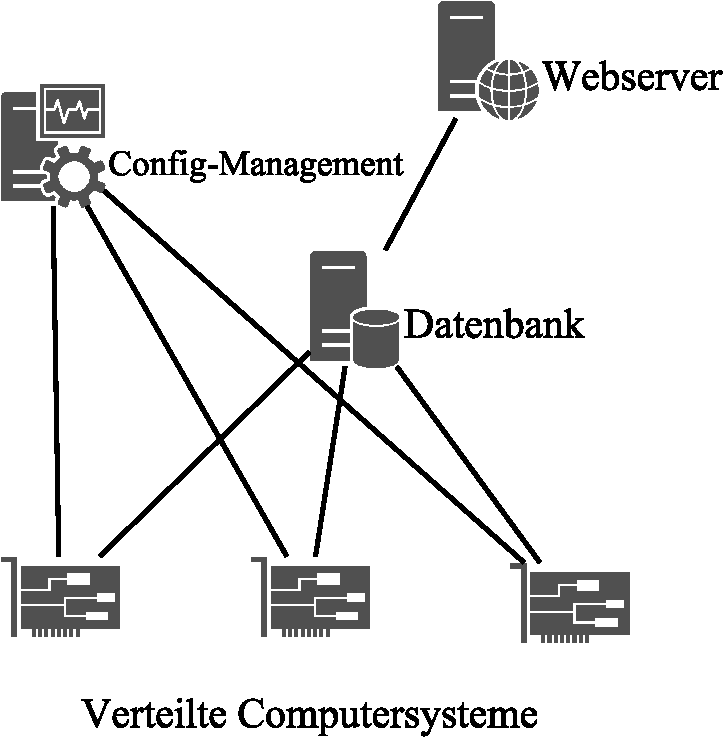
\includegraphics[width=0.5\textwidth]{figures/network.pdf}
    \caption{Netzwerk-Grundriss des Projekts}\label{fig:1}
\end{figure}

\section*{Danksagung}
Ich danke dem Rechenzentrum der TU Clausthal, dass ich dort meine
Bachelor-Arbeit schreiben darf.
\end{document}
